% vim: tw=78 encoding=utf8 ts=2 sw=2 expandtab softtabstop=2
\documentclass[11pt,twocolumn,a4paper,english]{article}

\usepackage[utf8]{inputenc}
\usepackage{babel}
\usepackage{url}
\usepackage{graphicx}
\usepackage{anysize}
\marginsize{1.7cm}{1.7cm}{1.7cm}{1.7cm}

\newcommand{\TODO}{\textbf{TODO:} }

\title{
Synthesizing Benchmarks for Architecture Recovery Algorithms}
\author{Rodrigo Souza \\ rodrigorgs@gmail.com 
\and Dalton Guerrero \\ dalton@dsc.ufcg.edu.br
\and Jorge Figueiredo \\ abrantes@dsc.ufcg.edu.br
\and Christina Chavez \\ flach@ufba.br
}

\begin{document}

\sloppy
\maketitle

\TODO Redo some figures to fit better in a two column paper.

\TODO Display authors in a 2x2 matrix.

\begin{abstract}
	As a software system evolves, its actual architecture may deviate from its original reference architecture. A better understanding of the actual architecture can be gained by applying architecture recovery algorithms to the source code of the system. Unfortunately, there is little knowledge regarding the quality of such algorithms, mostly because, in order to assess their accuracy, one needs updated, detailed architectures for a variety of software systems.
	To overcome such problem, we propose a simulation model that synthesizes implementation-level dependency graphs that conform to the module view of any given reference architecture. We show, using observations from network theory, that the graphs are very similar to dependency graphs extracted from the source code of real software systems. 
	Then, we synthesize thousands of graphs, in a controlled way, and use them as benchmarks for six well-known architecture recovery algorithms: ACDC, Bunch, SL75, SL90, CL75, and CL90. By comparing the given reference architectures with those recovered by the algorithms, we conclude that ACDC and Bunch outperform the alternatives, specially if the architecture contains more than a couple of modules.\end{abstract}

%%%%%%%%%%%%%%%%%%%%%%%%%%%%%%%%%%%%%%%%%%%%%%%%%%%%%%%%%%%%%%%%%%%%%%%%%%%%%
%%%%%%%%%%%%%%%%%%%%%%%%%%%%%%%%%%%%%%%%%%%%%%%%%%%%%%%%%%%%%%%%%%%%%%%%%%%%%

% I use begin/end instead of just \section so I can fold sections in my text editor
\begin{section}{Introduction}
% This section should be succinct, with no subheadings
	Architectural drift

	Reverse engineering / Architecture recovery algorithms
	
\end{section}

%%%%%%%%%%%%%%%%%%%%%%%%%%%%%%%%%%%%%%%%%%%%%%%%%%%%%%%%%%%%%%%%%%%%%%%%%%%%%

\begin{section}{Background}
	Architecture recovery algorithms

	Evaluation of architecture recovery algorithms. 
	
\end{section}

%%%%%%%%%%%%%%%%%%%%%%%%%%%%%%%%%%%%%%%%%%%%%%%%%%%%%%%%%%%%%%%%%%%%%%%%%%%%%

\begin{section}{The BCR+ model}	
	\newcommand{\din}[0]{\ensuremath{\delta_{in}}}
	\newcommand{\dout}[0]{\ensuremath{\delta_{out}}}
	\newcommand{\gin}[0]{\ensuremath{\mathrm{g}_{in}}}
	\newcommand{\gout}[0]{\ensuremath{\mathrm{g}_{out}}}
	
	\TODO Talk about network theory / complex networks / scale-free networks	

	When designing the architecture of a software system, the module viewpoint plays a major role, by specifying the modules of the system and their inter-relationships. Constraining such dependencies benefits the maintenatibility, portability, and reusability of the software system.
	
	In this section, we describe the BCR+ model for synthesizing graphs from a description of the module viewpoint of an arbitrary architecture --- that is, the modules and dependencies between modules. The BCR+ model produces---by means of the mechanisms of growth and preferential attachment---directed graphs that are both scale-free and segmented in modules.
	
	\TODO there are other models, but they don't take architecture as input	
	
\begin{subsection}{Overview}
	The BCR+ model is a generalization of a graph model proposed by Bollobás et al \cite{Bollobas2003}. The original model generates directed graphs that are scale-free. Our model extends the original by generating graphs in which the nodes are organized in modules, according to an modular architecture given as input.
	
	The BCR+ model takes the following parameters as input:
	
	\begin{itemize}
  \item number of vertices, $n$;
  \item three probability values, $p_1$, $p_2$ e $p_3$, com $p_1 + p_2 + p_3 = 1$;
  \item base in-degree, $\din$;
  \item base out-degree, $\dout$.
  \item an directed graph representing dependencies between modules, $G$;
  \item a constant, $\mu$, with $0,0 \le \mu \le 1,0$;
  \end{itemize}
  
	The last two parameters are new in BCR+. The other ones are from the original model by Bollobás et al \cite{Bollobas2003}.
	
	In the graph $G$, each vertex represents one module of the architecture. Each edge defines a relationship of dependency between modules. We say that a module $M_1$ depends on another module, $M_2$, if $G$ contains an edge from the vertex that represents $M_1$ to the vertex that represents $M_2$. In the graph that is created, an edge from a vertex $v_1 \in M_1$ to another vertex, $v_2 \in M_2$, can be created only if $M_1$ depends on $M_2$ in the graph $G$ or if $M_1$ and $M_2$ are the same module.
	
		\TODO Say that these graphs contain both internal and external edges. Define internal/external.
		
	The parameter $\mu$ controls the proportion of external edges in the graph---that is, edges connecting vertices in distinct modules. Lower values lead to graphs with fewer external edges.
	
	The original model by Bollobás et al \cite{Bollobas2003} is a particular case of BCR+ when $\mu = 0$ and $G$ contains one single vertex, representing one single module.
	

\begin{figure*}[htbp]
	\centering
		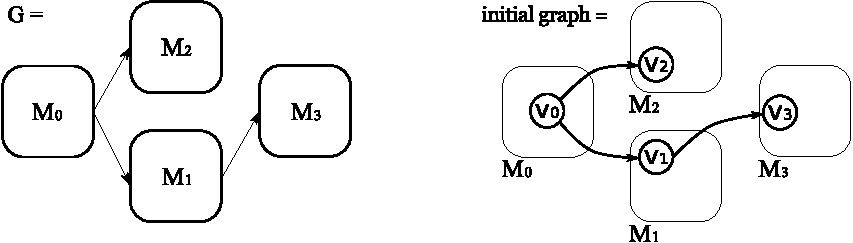
\includegraphics[scale=1]{figures/bcr-initial-graph}
	\caption{Initial graph synthesized by BCR+, given an input graph parameter $G$.}
	\label{fig:bcr-initial-graph}
\end{figure*}
	
	As a computer model, BCR+ takes the parameters as inputs and, by running an algorithm, outputs a graph. The algorithm builds the output graph incrementally. It starts by creating a module for each vertex in the input graph $G$, and then adding one vertex to each module. After that, it creates all external edges that are allowed by $G$ (see Figure \ref{fig:bcr-initial-graph}). Then, the graph is modified according to three formation rules that are applied successively, in random order, until the graph grows to $n$ vertices. At each algorithm step, the probability of the $i$-th being applied is given by the parameter $p_i$.

\end{subsection}	

\begin{subsection}{Formation Rules}
	
	There are three formation rules in BCR+. Each one modifies the output graph by adding or removing vertices or edges in the graph. Also, each formation rule has a probability of being applied, given by the parameters $p_1$, $p_2$ and $p_3$.

\begin{figure*}[htbp]
	\centering
		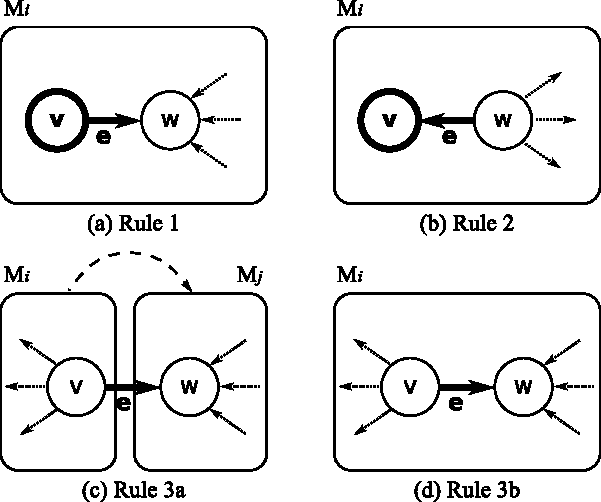
\includegraphics[scale=1]{figures/bcr-rules}
	\caption{Formation rules for BCR+. $M_i$ and $M_j$ are distinct modules, such as $M_i$ depends on $M_j$. In the diagram for each rule, thicker lines represent vertices and edges created when the rule is applied.}
	\label{fig:bcr-rules}
\end{figure*}

	The rules are illustrated in Figure \ref{fig:bcr-rules}. Simplified rules:
	
	\begin{itemize}
		\item Rule 1: one vertex is added to some module, together with an outgoing edge to another vertex in the same module.
		\item Rule 2: one vertex is added to some module, together with an ingoing edge coming from another vertex in the same module.
		\item Rule 3: one edge is added between two pre-existing vertices. There are two variations of this rule:
		\begin{itemize}
			\item Rule 3a: choose vertices from distinct modules.
			\item Rule 3b: choose vertices that are in the same module.
		\end{itemize}
	\end{itemize}
	
	The rules 1, 2, and 3b come directly from the original model by Bollobás et al \cite{Bollobas2003}. The rule 3a was created in BCR+ to account for inter-module dependencies.
	
	The choice of vertices to which add edges to is done according to preferential attachment. When we say that a vertex ``chosen according to $\mathrm{f}(x)$'', we mean that the probability of choosing the vertex $x$ is proportional to $\mathrm{f}(x)$:
	
	$$
	  \mathrm{P}(x) ~=~ \frac{ \mathrm{f}(x) }
	  { \displaystyle\sum_{i} \mathrm{f}(i) }
	$$
	
	The denominator is a normalization factor, such as the sum of probabilities $\mathrm{P}(x)$ is 1.
	
	With this definition in mind, the rules can be fully specified:
	
	\begin{itemize}
		\item Rule 1: \emph{Add a vertex with an outgoing edge}. An existing vertex, $w$, is chosen according to $\mathrm{f}(x) = \din + \gin(x)$ (that is, parameter $\din$ added to the vertex in-degree). A new vertex, $v$, is added to the module that contains $w$, together with an edge from $v$ to $w$.

		\item Rule 2: \emph{Add a vertex with an ingoing edge}. An existing vertex, $w$, is chosen according to $\mathrm{f}(x) = \dout + \gout(x)$. A new vertex, $v$, is added to the module that contains $w$, together with an edge from $w$ to $v$.

		\item Rule 3: \emph{Add an edge between pre-existing vertices}. A vertex, $v$, is chosen according to $\mathrm{f}(x) = \dout + \gout(x)$. Then, an edge is added from $v$ to another vertex, $w$, chosen according to $\mathrm{f}(x) = \din + \gin(x)$. The vertex $w$ is not chosen among the set of all vertices. In fact, there are two rules, and the choice of the rule to apply is probabilistic and depends on the parameter $\mu$:

		\begin{itemize}
		  \item Rule 3a: with proability $\mu$, $w$ is chosen among the vertices that are in modules on which the module of $v$ depends, according to the parameter $G$.
		  \item Rule 3b: with probability $1 - \mu$, $w$ is chosen among the vertices that are in the same module as $v$.
		\end{itemize}
	\end{itemize}
	
	\TODO BCR+ is a growth model, can simulate the evolution of a software system subject to constraints in module interaction. See CSMR paper (extended version), pg 2, col 2, just before section B. 
	
\end{subsection}

\begin{subsection}{Example}
	\TODO Do we need an Example section?
\end{subsection}
	
\end{section}

%%%%%%%%%%%%%%%%%%%%%%%%%%%%%%%%%%%%%%%%%%%%%%%%%%%%%%%%%%%%%%%%%%%%%%%%%%%%%

\begin{section}{Software-Realism}
	% Motifs / Triads. Triad concentration profiles.
	% Software-realism metric.
	% Software-realism classifier. Training and testing the classifier.
	% Software-realism for the BCR+ model. (Cite previous paper, where we also evaluate software-realism for three other models)
	
	If synthetic graphs built with BCR+ are to be used as surrogates to dependency graphs extracted from the source code of software systems, it is expected that they resemble such graphs. The property of a graph to resemble software dependency graphs is what we call software-realism. Hence, we seek to prove that BCR+ produces software-realistic graphs.
	
	\TODO Maybe, redo the analysis using neural networks and eliminate the need of a software-realism metric. (Or, maybe, a linear regression with up to quadratic terms is enough. Try both.)
	
	To this end, we propose a classifier---based on a software-realism metric---that, given a graph, outputs whether it is software-realistic or not. Then, we show that this classifier accurately classifies a data set consisting of both software-realistic graphs (extracted from open source software systems) and non software-realistic graphs (extracted from data studied in other domains). Finally we show that, with a suitable configuration of parameters, BCR+ can be used to synthesize software-realistic graphs.
	
	% In fact, we expect synthetic graphs to be indistinguishable from dependency graphs in all aspects that are relevant for graph-based architecture recovery algorithms. For this purpose, we chose to devise a classifier that distinguishes software dependency graphs from other graphs.
	
	% To capture this software quality of a graph, we define the concept of software-realism, that indicates to what extent a graph resembles software dependency graphs.
	
	% A metric for software-realism should be consistent, that is, it should present high values when measuring dependency graphs, and low values when measuring graphs from other domains---e.g., protein interaction networks, social networks etc.
	
	% First, we define a metric for software-realism, based on structural properties of a graph. Then, we show that the metric is consistent, by applying it to both software dependency graphs and graphs from non-software domains. After that, we build a classifier, based on the software-realism metric, that can be used to distinguish software dependency graphs from other graphs. Finally, we show that the BCR+ model is capable of synthesizing graphs with a high degree of software-realism, indistinguishable from software dependency networks.

\begin{subsection}{Data Set}
	\TODO Where to put this section?
	
	\begin{enumerate}
		\item Data collection: graphs and software systems
		\item Data preprocessing: extraction of software dependency graphs
		\item Data analysis: training and testing of the neural network
		\item Finally: classification of graphs synthesized by BCR+.
	\end{enumerate}
	
\end{subsection}

\begin{subsection}{Triad Concentration Profiles}
	
	Before presenting the graph classifier, we introduce the concept of triads and triad concentration profiles. Given three vertices, one can conceive 13 distinct connected directed graphs---the so-called triads---, as shown in Figure \ref{fig:triads}. By counting how often each triad appears in a graph, one can build a 13-dimension vector that is called triad concentration profile. % it's like the signature for a graph.

	\begin{figure*}[htbp]
		\centering
			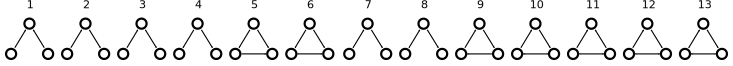
\includegraphics[scale=1]{figures/triads}
		\caption{All triads---connected directed graphs with three vertices---, numbered from 1 to 13.}
		\label{fig:triads}
	\end{figure*}
	
	Previous work has shown that graphs from the same domain tend to be caracterized by similar triad concentration profiles \cite{Milo2002}. For example, Figure \ref{fig:triads}(a) presents triad concentration profiles for two software dependency graphs, whereas Figure \ref{fig:triads}(b) presents triad concentration profiles for graphs in distinct domains: a software dependency graph and a linguistic graph. An informal analysis reveals that the similarity between the profiles is greater in the first case. It should suffice to notice that, in the second case, the concentration of the first two triads is somewhat reversed (in the linguistic graph, the second triad is the most frequent).

	\begin{figure*}[htbp]
		\centering
			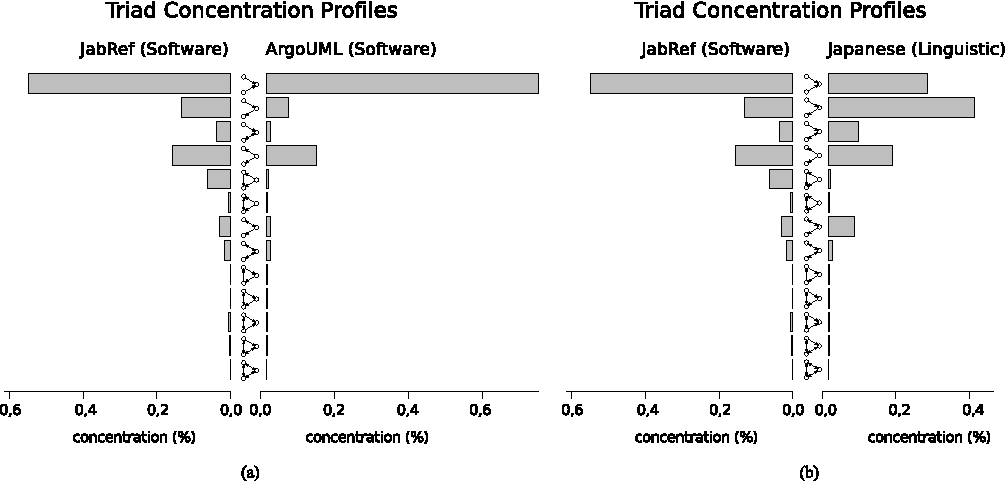
\includegraphics[scale=1]{figures/tcp}
		\caption{Comparison between triad concentration profiles for three distinct graphs (computed with the igraph tool \cite{igraph}). (a) Class dependency graphs for two softwares: JabRef, version 2.5b2 (left) and ArgoUML version 0.28 (right). (b) Graph for JabRef, version 2.5b2 (left), and graph of word succession in a sample of Japanese texts (right) \cite{Milo2004}.}
		\label{fig:tcp}
	\end{figure*}
	
	Many authors \cite{Milo2004,Ma2007,Lin2008} have explored the use of Pearson's correlation coefficient on triad concentration profiles in order to find clusters of structurally similar graphs. The results suggest that the technique is effective in identifying groups of graphs from the same domain (e.g., social, linguistic, biologic etc.).
			
	\end{subsection}
	
\begin{subsection}{Software-Realism Metric}
%	Based on triad concentration profiles, we define the software-realism metric, that is fundamental to the graph classifier.

	We define the similarity between two graphs to be the correlation between the corresponding triad concentration profiles:
	
	$$
  \mathrm{sim}(a, b) ~=~ 
    \mathrm{cor}(\mathrm{PCT}(a), \mathrm{PCT}(b))\mathrm{.}
  $$
	
	\TODO I could have just trained a neural network with our extended training set (software graphs + graphs from other domains).
	
	To define a software-realism of a graph, $x$, we rely on the similarity metric and on a data set, $R$, containing graphs that are considered software-realistic. The software-realism, $\mathrm{S}(x, R)$, is defined as the average similarity between $x$ and each of the graphs in the reference data set, $R$:
		
	$$
  \mathrm{S}(x, R) ~=~ \frac{
  \displaystyle\sum_{s \in R} \mathrm{sim}(x, s)
  }{|R|} \mbox{.}
  $$

\end{subsection}
	
\begin{subsection}{Metric Evaluation}
	
	\TODO Classification model:
	
	$$
	  \mathrm{m}(x, R, S_0) ~=~
	  \left\{
	  \begin{array}{cl}
	  \mbox{sw-realistic,} & \mbox{se } \mathrm{S}(x, R) \ge S_0; \\
	  \mbox{non sw-realistic,} & \mbox{caso contrário.}
	  \end{array}
	  \right.
	$$	
	
	\TODO data collection; data processing (extracting dependency graphs); analysis (accuracy, precision, recall)
	
	\TODO choice of $S_0$.
	
\end{subsection}
	
\begin{subsection}{Software-Realism of BCR+}
	\TODO choice of parameters; graph synthesizing; graph classification (according to sw-realism)
\end{subsection}
	
\end{section}

%%%%%%%%%%%%%%%%%%%%%%%%%%%%%%%%%%%%%%%%%%%%%%%%%%%%%%%%%%%%%%%%%%%%%%%%%%%%%

\begin{section}{Evaluation of Architecture Recovery Algorithms}
	\TODO Clustering

	\TODO Brief description about Bunch, ACDC, SL75/SL90, CL75, CL90
	
	\TODO Traditional experimental setup for evaluation of architecture recovery algorithms: given a dependency graph and a reference architecture, run the algorithm on the graph and compare the recovered architecture with the reference architecture.
	
	\TODO MoJo metric.

\begin{subsection}{Experimental Setup}
	\TODO Section 6.3 from dissertation
\end{subsection}

\begin{subsection}{Comparison of Architecture Recovery Algorithms}
	% Section 6.4 from dissertation
	
	The first experiment was aimed at comparing the performance of the algorithms when applied software-realistic graphs, measured by the similarity between the clusters found by the algorithms and the modules of the reference architecture.
	
	We have selected for this experiment only the graphs that were classified as software-realistic, totalizing about 6,000 graphs. Then, each algorithm was applied to each one of the synthetic graphs, resulting in a set of clusters together with a mapping from the set of vertices to the set of clusters. The performance of the clusterings were measured with the metric MoJoSim.
	
	The Figure \ref{fig:exp-algorithms} shows a boxplot of the MoJoSim values that were measured for each algorithm. The dashed lines indicate the maximum and minimum value from the data. Comparing the median performance of the algorithms, it is clear that ACDC presents the best performance, followed by Bunch, and then by the hierachical algorithms. These differences were verified to be significative by applying a paired Wilcoxon test ($\alpha = 0.05$), with Bonferroni correction to account for multiple hypothesis testing. Among the hierarchical algorithms, there was no evidence that their performances differ.
	
	\begin{figure}[htbp]
		\centering
			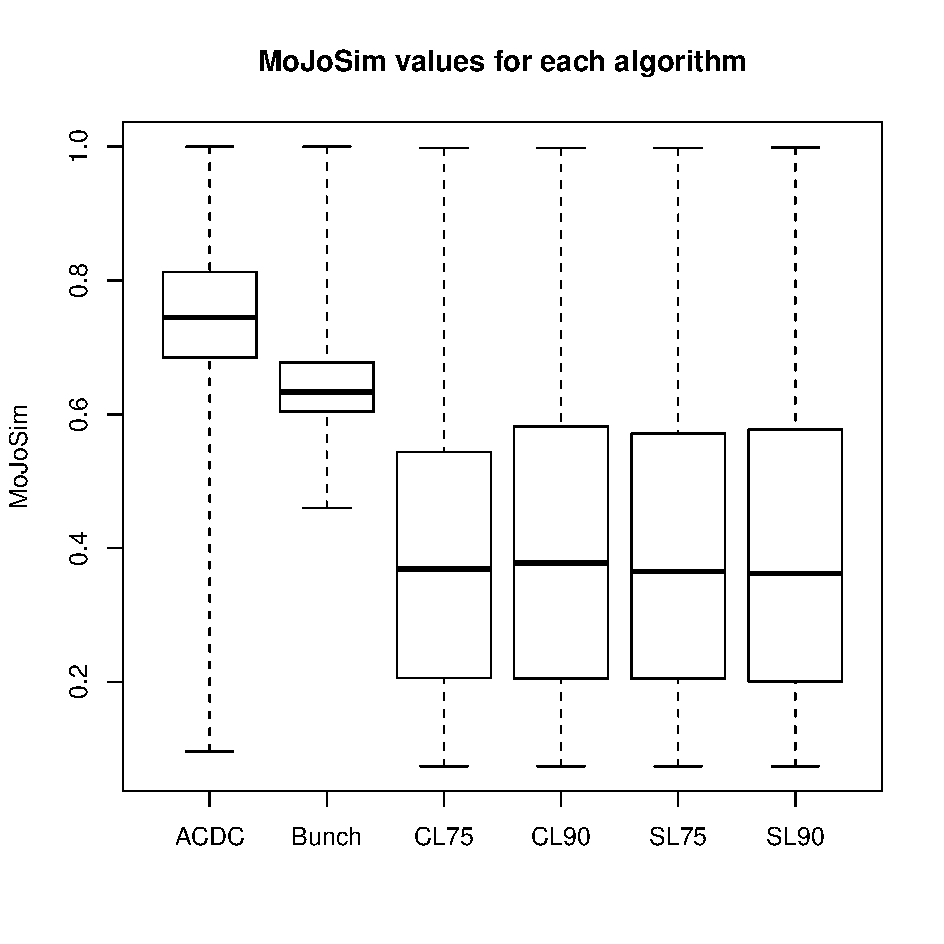
\includegraphics[scale=0.5]{figures/exp-algorithms}
		\caption{Statistical summary of MoJoSim values for each architecture recovery algorithm.}
		\label{fig:exp-algorithms}
	\end{figure}
	
	Another noteworthy aspect of the data is the dispersion of values. The algorithm Bunch presents the smaller dispersion, with more that half of the values between 0.60 and 0.80 (minimum value = 0.45). In the case of ACDC, half of the values are between 0.65 a 0.85, but the minimum value is 0.01. This observation suggests that, although Bunch presents overall inferior performance when compared with ACDC, it can be a resonable choice for yielding more predictable results.
	
	\TODO move to a discussion section.
	The results disagree with conclusions from Wu, Hassah, and Holt \cite{Wu2005}. They have concluded that the SL algorithms outperform ACDC, which outperforms Bunch, which outperforms the CL algorithms. The disagreement probably can be explained by the criteria they used to build the reference architecture for each software system. They use the folder structure from the source of the software system to determine the modules in the architecture reference. In our work, the reference architecture is defined a priori, and the graphs are synthesized ro reduce the dependencies between modules.
	
	We should note that this experiment suffers from sampling bias. Although all analyzeds graphs are software-realistic, we can not guarantee that it is representative of all software systems. We see this analysis as complementary to similar experiments, that suffer from other types of bias \cite{Wu2005,Bittencourt2009,Andritsos2005}.
	
\end{subsection}	

\begin{subsection}{Algorithm Parameters Analysis}
	% Section 6.5 from dissertation
	
	In the next experiment, we tried to understand how the algorithms behave on a variety of situations---graphs with different number of modules, different proportions of external edges etc. We were able to control a number of graph properties by changing parameter values for the BCR+ model.
	
	In this experiment, all graphs---both software-realistic and non software-realistic---were considered, in order to avoid the software-realism variable to bias the results.
	
	We have analyzed the influence of the number of modules and of the proportion of external edges on the performance of the algorithms. We have chosen these two properties because they map naturally to BCR+ parameters: number of modules is controlled by the input module graph, $G$, and proportion of external edges is controlled by the parameter $\mu$.

	\TODO explain that the sample is paired, that is, there are two graphs that differ only by $\mu$ (the other parameters are identical).
	
	\TODO this experiment is not possible with traditional approaches, since it depends on having control on the graphs properties.
	
	As expected, all algorithms performed better when the proportion of external edges was smaller. \TODO is it true? Check experimental package
	
	A surprising result was found when analyzing the influence of the number of modules on the performance of the algorithms (see Figure \ref{fig:exp-number-modules}). While the performance of ACDC and Bunch are not influenced by the number of modules, the performance of the hierachical algorithms is worse when applied to graphs with more modules. In fact, the performance of such algorithms are comparable to the performance of ACDC and Bunch when there are only two modules, but it gets  progressively worse as the number of modules grows.
	
	\begin{figure}[htbp]
		\centering
			
\includegraphics[scale=0.5]{figures/exp-number-modules}
		\caption{Influence of the number of modules in the reference architecture on the performance of each architecture recovery algorithm.}
		\label{fig:exp-number-modules}
	\end{figure}
	
	A possible explanation for this phenomenom can be found in the distribution of module sizes found by hierarchical algorithms. It is common that they found large modules, sometimes covering more than half of the vertices \cite{Wu2005}. If the reference architecture contains many smaller modules, large modules found by an algorithm are severely penalyzed by the MoJoSim metric (the large modules need to be split in smaller modules, which is accounted in MoJoSim as a sequence of vertex movimentations).
	
\end{subsection}

\begin{subsection}{Impact of Bidirectional Dependencies}
	% Section 6.6 from dissertation
	
	The third experiment was aimed at measuring the influence of the type of dependency (unidirectional of bidirectional) on the performance of each architecture recovery algorithm. The independent variable is the parameter $G$ from BCR+, that is, the definition of the modules and allowed dependencies between modules.
	
	We have analyzed two configurations for $G$:
	
	\begin{itemize}
		\item \emph{bidirectional}: $G$ contains two modules, $M_1$ and $M_2$; there is a bidirectional edge between $M_1$ and $M_2$ (that is, vertices in $M_1$ may depend on vertices of $M_2$ and the other way around);
		
		\item \emph{unidirectional}: $G$ contains two modules, $M_1$ and $M_2$; there is an unidirectional edge from $M_1$ to $M_2$ (that is, vertices in $M_1$ may depend on vertices of $M_2$, but the opposite is not true).
	\end{itemize}
	
	As far as we know, BCR+ is the only graph model that can be used to conduct this type of experiment. Other graph models do not offer control over specific dependencies.
	
	For the remaining parameters of BCR+, when considered the values described in Section XXX. For each configuration of parameters, three graphs were synthesized, totalizing 11,400 graphs. Then, each architecure recovery algorithm was applied to each graph. Finally, the performance was computed, using the metric MoJoSim.
	
	The results are shown in a boxplot in Figure \ref{fig:exp-dependencies}. It can be observed that all algorithms performed slightly better on the graph with the unidirectional edge. All differences---except that of CL75---are significative at 5\% level, as assessed with the paired Wilcoxon test.
	
	\begin{figure*}[htbp]
		\centering
			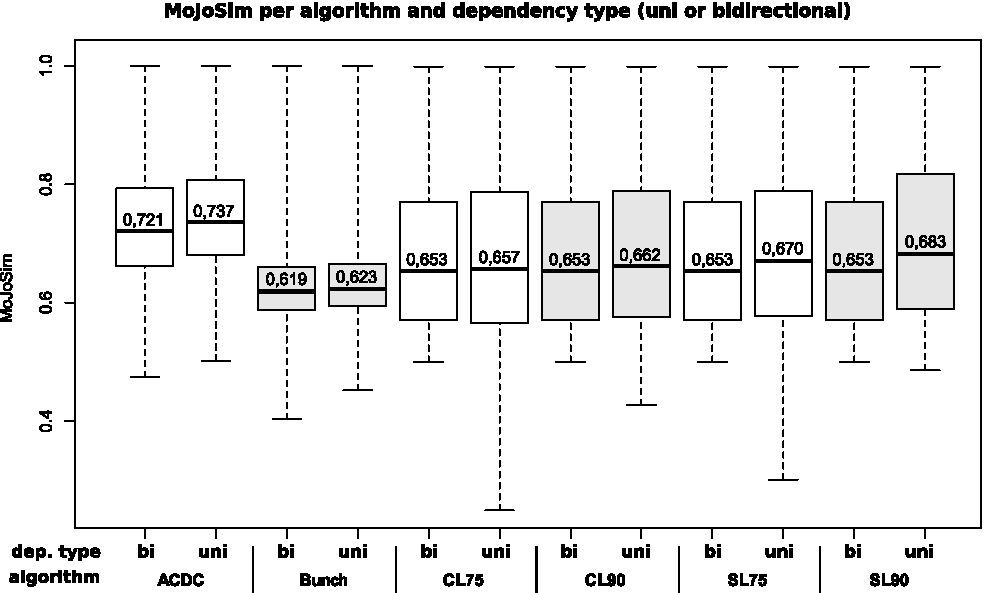
\includegraphics[scale=1]{figures/exp-dependencies}
		\caption{Influence of the type of dependency between modules (unidirectional ou bidirectional) on the performance of each architecture recovery algorithm.}
		\label{fig:exp-dependencies}
	\end{figure*}
	
	The difference of performance for each algorithm is shown in Table \ref{tab:exp-dependencies}, as a 95\% confidence interval. ACDC and SL75 are more influenced by the choice of dependency type than the other algorithms. Overall, the difference between MoJoSim values does not exceed 0.03 (except in the case of SL90), which is a small value.
	
	\begin{table*}[width=\textwidth]
	  \begin{center}
	  \begin{tabular}{cccccc}
	    \hline
	    \textbf{ACDC} & \textbf{Bunch} & \textbf{CL75} & \textbf{CL90} & \textbf{SL75} & \textbf{SL90} \\
	    \hline
	    \hline
	    \footnotesize{[0,016; 0,023]} & \footnotesize{[0,004; 0,008]} & \footnotesize{[-0,004; 0,006]} & \footnotesize{[0,006; 0,015]} & \footnotesize{[0,007; 0,017]} & \footnotesize{[0,021; 0,031]} \\
	    \hline
	  \end{tabular}
	  \end{center}
	  \caption{Intervalo de confiança de 95\% para a diferença de desempenho de cada algoritmo, medido em MoJoSim, entre a configuração \emph{simples} e a configuração \emph{dupla} do parâmetro G.}
	  \label{tab:exp-dependencies}
	\end{table*}
	
	We conclude that, in general, the presence of modules with mutual, bidirectional dependencies, influences negatively the performance of the algorithms that were analyzed. The observed difference was small in our study with two modules, but we suspect that this difference can be greater on graphs with more modules and more bidirectional dependencies.
	
\end{subsection}

\begin{subsection}{Discussion}
	We have described three experiments based on the application of architecture recovery algorithms to synthetic graphs created by the model BCR+. The experiments present evidence that this approach is practicable and can be used to find insights about the algorithms that cannot be found with more traditional approaches.
	
	\TODO more
	
\end{subsection}

\end{section}

%%%%%%%%%%%%%%%%%%%%%%%%%%%%%%%%%%%%%%%%%%%%%%%%%%%%%%%%%%%%%%%%%%%%%%%%%%%%%

\begin{section}{TODO: Other Possible Sections}
	Discussion
	
	Limitations
	
	Conclusion
	
	Acknowledgments
	
	References	
\end{section}

%%%%%%%%%%%%%%%%%%%%%%%%%%%%%%%%%%%%%%%%%%%%%%%%%%%%%%%%%%%%%%%%%%%%%%%%%%%%%
%%%%%%%%%%%%%%%%%%%%%%%%%%%%%%%%%%%%%%%%%%%%%%%%%%%%%%%%%%%%%%%%%%%%%%%%%%%%%

\bibliographystyle{plain}
\bibliography{ase2012-reference-arch}

\end{document}
